\documentclass{article}
\usepackage[a4paper, left=25.4mm, top=25.4mm, right=25.4mm, bottom=25.4mm]{geometry}
\usepackage[shortlabels]{enumitem}
\usepackage{amsmath}
\usepackage{amssymb}
\usepackage{amsthm}
\usepackage{authoraftertitle}
\usepackage{blindtext}
\usepackage{booktabs}
\usepackage{bussproofs}
\usepackage{bm}
\usepackage{color}
\usepackage[dvipsnames]{xcolor}
\usepackage{fancyhdr}
\usepackage{graphicx}
\usepackage[hidelinks]{hyperref}
\usepackage{latexsym}
\usepackage{multicol}
\usepackage{newpxtext}
%\usepackage{newpxmath}
\usepackage{ragged2e}
\usepackage{subcaption}
\usepackage{textcomp}
\usepackage{textgreek}
\usepackage{vwcol}
\renewcommand{\headrulewidth}{0pt}
\renewcommand{\qedsymbol}{Q.E.D.}
\renewcommand{\sfdefault}{lmss}
\renewcommand{\thesubsection}{\arabic{subsection}}

\author{Victor Zhao\\xz398@cam.ac.uk}

\begin{document}
\centering
\section*{Representation Learning on Graphs and Networks (L45)\\CST Part III / MPhil in ACS}
\MyAuthor

\justifying

\subsection{Primer on Graph Representations}

\begin{enumerate}
	\item Mathematical definition of graphs: 
	
	A \textit{graph} $\mathcal{G}=(\mathcal{V}, \mathcal{E})$ is a collection of nodes $\mathcal{V}$ and edges $\mathcal{E}\subseteq\mathcal{V}\times\mathcal{V}$
	
	The edges can be represented by an \textit{adjacency matrix}, $\mathbf{A}\in\mathbb{R}^{|\mathcal{V}|\times|\mathcal{V}|}$, such that
	$$A_{uv}=\begin{cases}
		1 &\text{if }(u,v)\in\mathcal{E}\\
		0 &\text{otherwise}
	\end{cases}$$

	\item Some interesting graph types:
	\begin{itemize}[topsep=0pt]
		\item \textbf{Undirected}: $\forall u, v\in\mathcal{V}.\ (u,v)\in\mathcal{E}\Longleftrightarrow (u,v)\in\mathcal{E}$ (i.e., $\mathbf{A}^\top=\mathbf{A}$)
		\item \textbf{Weighted}: provided \textit{edge weight} $w_{uv}$ for every edge $(u,v)\in\mathcal{E}$
		\item \textbf{Multirelational}:~various~\textit{edge~types},~i.e.~$(u,t,v)\in\mathcal{E}$~if~there~exists~an~edge~$(u,v)$~linked~by~type~$t$
		\item \textbf{Heterogeneous}: various \textit{node types}
	\end{itemize}

	\item Machine learning tasks on graphs by domain:
	\begin{itemize}[topsep=0pt]
		\item \textbf{Transductive}: training algorithm sees all observations, including the holdout observations
		\begin{itemize}[topsep=0pt]
			\item Task is to \textit{propagate} labels from the training observations to the holdout observations 
			\item Also called \textit{semi-supervised learning}
		\end{itemize}
		\item \textbf{Inductive}: training algorithm only sees the training observations during training, and only sees the holdout observations for prediction
	\end{itemize}

	\item Node statistics:
	\begin{itemize}[topsep=0pt]
		\item \textbf{Degree}: amount of edges the node is incident to:
		$$d_u=\sum_{v\in\mathcal{V}}A_{uv}$$
		\item \textbf{Centrality}: a measure of how ``central'' the node is in the graph: how often do infinite random walks visit the node?
		$$d_u=\lambda^{-1}\sum_{v\in\mathcal{V}}A_{uv}e_v$$
		where $\mathbf{e}\in\mathbb{R}^{|\mathcal{V}|}$ is the largest eigenvector of $\mathbf{A}$, with corresponding eigenvalue $\lambda$
		\item \textbf{Clustering coefficient}: a measure of ``clusteredness'': are neighbours connected amongst each other?
		$$c_u=\frac{\left|\big\{(v_1, v_2)\in\mathcal{E}\big|v_1, v_2\in\mathcal{N}(u)\big\}\right|}{{d_u \choose 2}}$$
	\end{itemize}

%	\item Erd\H{o}s-R\'{e}nyi (ER) random graphs: modelling a data network $\mathcal{G}=(\mathcal{V}, \mathcal{E})$ with $|\mathcal{V}|=n$ and $|\mathcal{E}|=m$
%	\begin{itemize}[topsep=0pt]
%		\item Edges are added between pairs of nodes uniformly at random with the same probability $p$
%		\item Two equivalent methods for constructing ER graphs:
%		\begin{itemize}
%			\item $\mathcal{G}_{n,p}$: pick $p$ so that the resulting model network has $m$ edges
%			\item $\mathcal{G}_{n,m}$: pick randomly $m$ pairs of nodes and add edges between them
%			\item Degree distribution:
%			$$\Pr(\text{deg}(v)=k)={n-1 \choose k}p^k(1-p)^{(n-1)-k}$$
%			For $n\to\infty$, $np=\text{constant}$ and small $k$:
%			$$\Pr(\text{deg}(v)=k)\to\frac{(np)^k e^{-np}}{k!}\qquad\text{(Poisson distribution)}$$
%			\item $\text{Clustering coefficient}=p$
%		\end{itemize}
%	\end{itemize}

	\item Graph Laplacian:
	
	Let $\mathbf{D}$ be the diagonal (out)-degree matrix of the graph, i.e., $D_{uu}=\sum_{v\in\mathcal{V}}A_{ij}$. Then:
	\begin{itemize}[topsep=0pt]
		\item The \textit{unnormalised} graph Laplacian: $\mathbf{L}=\mathbf{D}-\mathbf{A}$
		\item The \textit{symmetric} graph Laplacian: $\mathbf{L}_\text{sym}=\mathbf{D}^{-\frac{1}{2}}\mathbf{L}\mathbf{D}^{-\frac{1}{2}}=\mathbf{I}-\mathbf{D}^{-\frac{1}{2}}\mathbf{A}\mathbf{D}^{-\frac{1}{2}}$
		\item The \textit{random walk} graph Laplacian: $\mathbf{L}_\text{RW}=\mathbf{D}^{-1}\mathbf{L}=\mathbf{I}-\mathbf{D}^{-1}\mathbf{A}$
	\end{itemize}
	
	Properties:
	\begin{itemize}[topsep=0pt]
		\item For undirected graphs, $\mathbf{L}$ is \textit{symmetric} ($\mathbf{L}^\top=\mathbf{L}$) and \textit{positive semi-definite} ($\forall\mathbf{x}\in\mathbb{R}^{|\mathcal{V}|}.\ \mathbf{x}^\top\mathbf{L}\mathbf{x}\geq0$)
		\item For undirected graphs:
		$$\forall \mathbf{x}\in\mathbb{R}^{|\mathcal{V}|}.\ \mathbf{x}^\top\mathbf{L}\mathbf{x}=\frac{1}{2}\sum_{u\in\mathcal{V}}\sum_{v\in\mathcal{V}}A_{uv}(x_u-x_v)^2=\sum_{(u,v)\in\mathcal{E}}(x_u-x_v)^2$$
		\item $\mathbf{L}$ has $|\mathcal{V}|$ nonnegative eigenvalues: $\lambda_1\geq\cdots\geq\lambda_{|V|}=0$
	\end{itemize}
	\newpage
	\item Spectral clustering:
	\begin{itemize}[topsep=0pt]
		\item Two-way cut: partition the graph into $\mathcal{A}\subseteq\mathcal{V}$ and its complement $\mathcal{A}_c\subseteq\mathcal{V}$:
		$$\text{Cut}(\mathcal{A})=\left|\big\{(u, v)\in\mathcal{E}\big|u\in\mathcal{A}\wedge v\in\mathcal{A}_c\big\}\right|$$
		\textit{Ratio cut} metric:
		$$\text{RCut}(\mathcal{A})=\text{Cut}(\mathcal{A})\left(\frac{1}{|\mathcal{A}|}+\frac{1}{|\mathcal{A}_c|}\right)$$
		\item Minimising $\text{RCut}(\mathcal{A})$:
		
		Let $\mathbf{a}\in\mathbb{R}^{|\mathcal{V}|}$ be a vector representing the cut $\mathcal{A}$, defined as follows:
		$$a_u=\begin{cases}
			\sqrt{\frac{\mathcal{A}_c}{\mathcal{A}}} &\text{if }u\in\mathcal{A}\\
			-\sqrt{\frac{\mathcal{A}}{\mathcal{A}_c}} &\text{if }u\in\mathcal{A}_c\\
		\end{cases}$$
		Then
		$$\mathbf{a}^\top\mathbf{L}\mathbf{a}=\sum_{(u,v)\in\mathcal{E}}(a_u-a_v)^2=|\mathcal{V}|\text{RCut}(\mathcal{A})$$
		Minimising $\mathbf{a}^\top\mathbf{L}\mathbf{a}$ corresponds to minimising $\text{RCut}(\mathcal{A})$ (NP-hard as the constraint is discrete)
		\item Relaxing: minimise $\mathbf{a}^\top\mathbf{L}\mathbf{a}$ subject to $\mathbf{a}\perp\mathbf{1}$ and $||\mathbf{a}||^2=|\mathcal{V}|$
		
		Rayleigh--Ritz Theorem: The solution is exactly the second-smallest eigenvector of $\mathbf{L}$
		
		To obtain the cut, place $u$ into $\mathcal{A}$ or $\mathcal{A}_c$ depending on the sign of $a_u$
		\item Can be generalised to $k$-clustering 
	\end{itemize}
\end{enumerate}

\subsection{Permutation Invariance and Equivariance}

\begin{enumerate}
	\item Informal definitions:
	\begin{itemize}[topsep=0pt]
		\item \textbf{Permutation invariance}: applying a permutation matrix does not modify the result
		\item \textbf{Permutation equivariance}: transformation preserves the node order
		\item \textbf{Locality}: signal remains stable under slight deformations of the domain
	\end{itemize}

	\item Setup:
	\begin{itemize}[topsep=0pt]
		\item \textbf{Node feature matrix}: $\mathbf{X}=\begin{bmatrix}
			\mathbf{x}_1 & \cdots & \mathbf{x}_{|\mathcal{V}|}
		\end{bmatrix}^\top\in\mathbb{R}^{|\mathcal{V}|\times k}$, where $\mathbf{x}_i\in\mathbb{R}^k$ is the features of node~$i$
		\item \textbf{(1-hop) neighbourhood} of node $i$: $\mathcal{N}_i=\big\{j\big|(i,j)\in\mathcal{E}\vee(j,i)\in\mathcal{E}\big\}$
		\item \textbf{Neighbourhood features}: $\mathbf{X}_{\mathcal{N}_i}=\{\!\{\mathbf{x}_j|j\in\mathcal{N}_i\}\!\}$
		\item \textbf{Permutation matrix}: a $|\mathcal{V}|\times|\mathcal{V}|$ binary matrix that has exactly one entry of 1 in every row and column, and 0s elsewhere: $\mathbf{P}=\begin{bmatrix}
			\mathbf{e}_{\pi(1)} & \cdots & \mathbf{e}_{\pi(|\mathcal{V}|)}
		\end{bmatrix}^\top$
	\end{itemize}

	\item Learning on sets:
	\begin{itemize}[topsep=0pt]
		\item $f(\mathbf{X})$ is \textit{permutation invariant} if for all permutation matrices $\mathbf{P}$: $f(\mathbf{PX})=f(\mathbf{X})$
		\item $\bm{F}(\mathbf{X})$ is \textit{permutataion equivariant} if for all permutation matrices $\mathbf{P}$: $\bm{F}(\mathbf{PX})=\mathbf{P}\bm{F}(\mathbf{X})$ 
		\item Locality on sets: transform every node in isolation, through a shared function $\psi$: $\mathbf{h}_i=\psi(\mathbf{x}_i)$
		
		Stacking $\mathbf{h}_i$ into a matrix yields $\mathbf{H}=\bm{F}(\mathbf{X})$:
		$$\bm{F}(\mathbf{X})=\begin{bmatrix}
			\text{---} & \!\!\!\psi(\mathbf{x}_1) & \!\!\!\text{{--}{--}} \\ 
			{} & \vdots & {} \\
			\text{{--}{--}} & \!\!\!\psi(\mathbf{x}_{|\mathcal{V}|}) & \!\!\!\text{{--}{--}}
		\end{bmatrix}$$
		\item Deep Sets (\href{https://papers.nips.cc/paper/2017/file/f22e4747da1aa27e363d86d40ff442fe-Paper.pdf}{Zaheer \textit{et al.}, NIPS 2017}):
		$$f(\mathbf{X})=\phi\left(\bigoplus_{i\in\mathcal{V}}\psi(\mathbf{x}_i)\right)$$
		Universality of Deep Sets: any permutation invariant model can be expressed as a Deep Sets
	\end{itemize}

	\item Learning on graphs:
	\begin{itemize}[topsep=0pt]
		\item $f(\mathbf{X})$ is \textit{permutation invariant} if for all permutation matrices $\mathbf{P}$: $f(\mathbf{PX},\mathbf{PA}\mathbf{P}^\top)=f(\mathbf{X},\mathbf{A})$
		\item $\bm{F}(\mathbf{X})$ is \textit{permutataion equivariant} if for all permutation matrices $\mathbf{P}$: $\bm{F}(\mathbf{PX},\mathbf{PA}\mathbf{P}^\top)=\mathbf{P}\bm{F}(\mathbf{X},\mathbf{A})$ 
		\item Locality on graphs: apply a local function $\phi$ over all neighbourhoods:
		$$\bm{F}(\mathbf{X},\mathbf{A})=\begin{bmatrix}
			\text{---} & \!\!\!\phi(\mathbf{x}_1,\mathbf{X}_{\mathcal{N}_1}) & \!\!\!\text{{--}{--}} \\ 
			{} & \vdots & {} \\
			\text{{--}{--}} & \!\!\!\phi(\mathbf{x}_{|\mathcal{V}|},\mathbf{X}_{\mathcal{N}_{|\mathcal{V}|}}) & \!\!\!\text{{--}{--}}
		\end{bmatrix}$$
		To ensure permutation equivariance, it is sufficient that $\phi$ is permutation invariant in $\mathbf{X}_{\mathcal{N}_i}$
	\end{itemize}
\end{enumerate}

\subsection{Graph Neural Networks}

\begin{enumerate}
	\item Graph Networks (\href{https://arxiv.org/pdf/1806.01261.pdf}{Battaglia \textit{et al.}, 2018}):
	
	Data flow:
	\begin{itemize}[topsep=0pt]
		\item Update edge features (using relevant nodes + graph)
		$$\mathbf{h}_{uv}=\psi(\mathbf{x}_u,\mathbf{x}_v,\mathbf{x}_{uv},\mathbf{x}_\mathcal{G})$$
		\item Update node features (using updated relevant edges + graph)
		$$\mathbf{h}_{u}=\phi\left(\mathbf{x}_u,\bigoplus_{u\in\mathcal{N}_v}\mathbf{h}_{uv},\mathbf{x}_\mathcal{G}\right)$$
		\item Update graph features (using updated nodes + edges)
		$$\mathbf{h}_\mathcal{G}=\rho\left(\bigoplus_{u\in\mathcal{V}}\mathbf{h}_{u},\bigoplus_{(u,v)\in\mathcal{E}}\mathbf{h}_{uv},\mathbf{x}_\mathcal{G}\right)$$
	\end{itemize}
	Visualisation (\textcolor{RoyalBlue}{\bf equivariant} and \textcolor{OrangeRed}{\bf invariant} layers):
	\begin{figure}[h]
		\centering
		\hspace*{4em}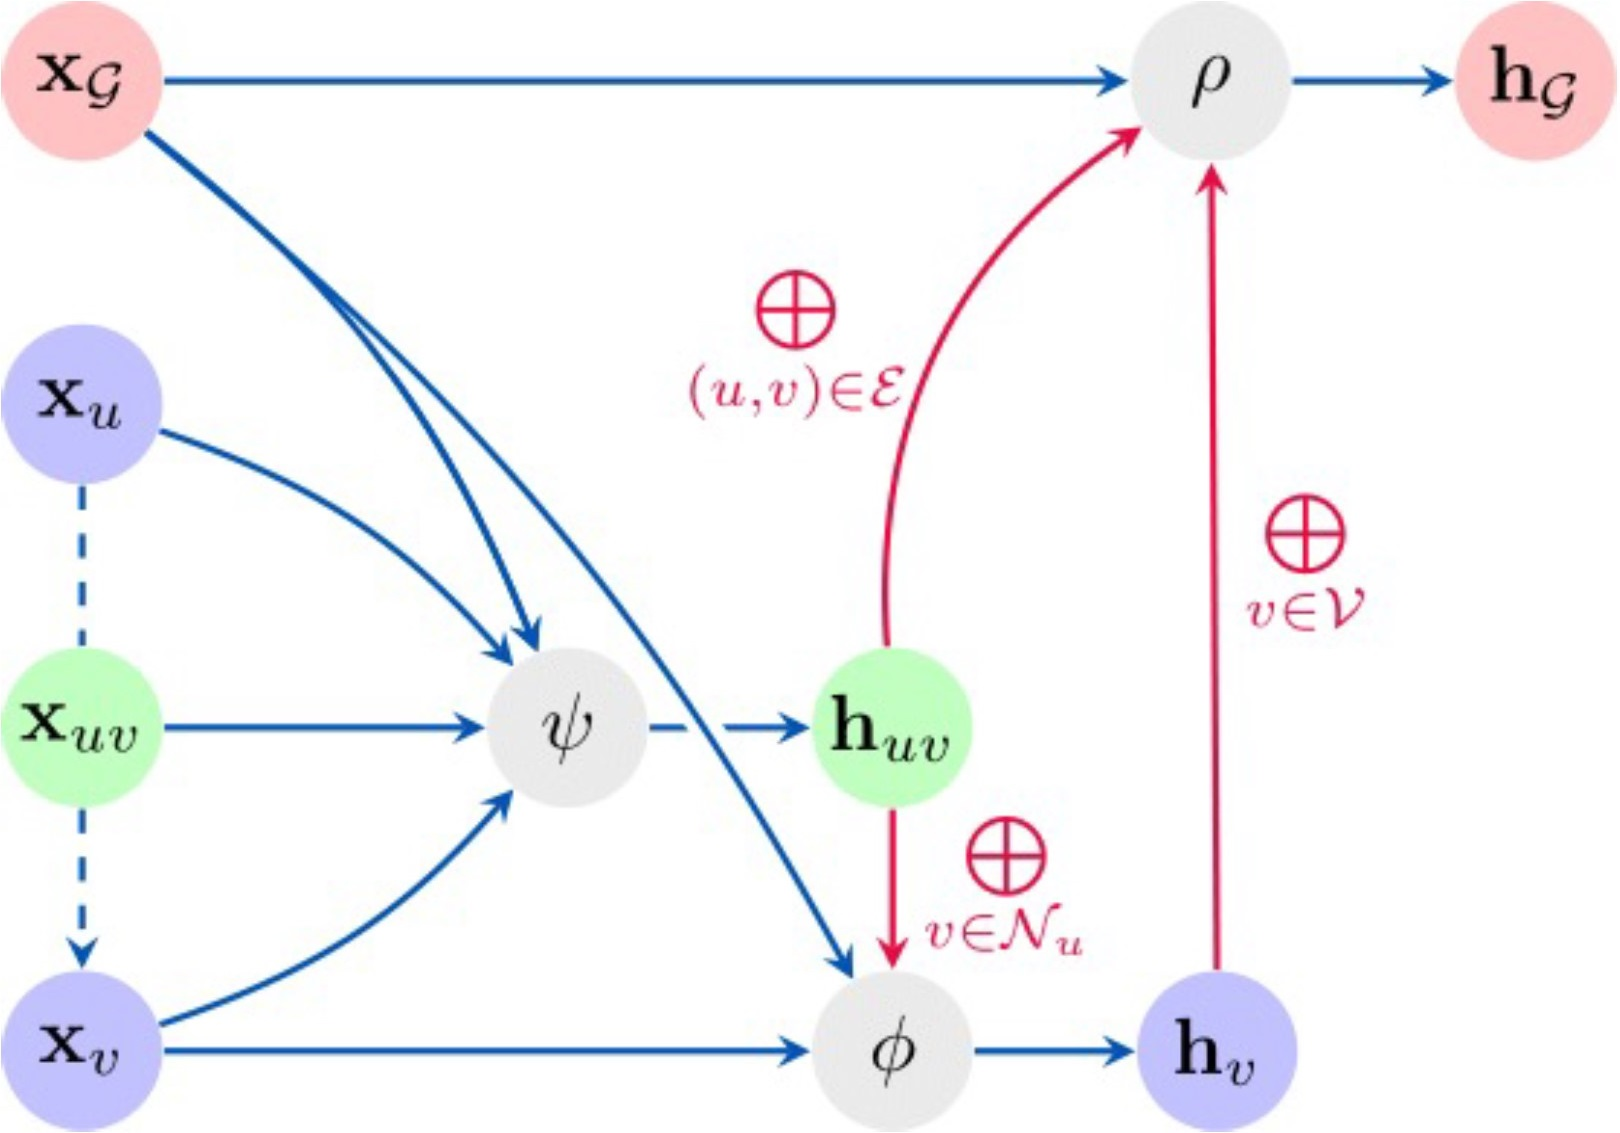
\includegraphics[width=0.4\textwidth]{figs/graph-network}
	\end{figure}

	\item Three flavours of GNN layers:
	\begin{figure}[h]
		\centering
		\begin{subfigure}[b]{0.3\textwidth}
			\centering
			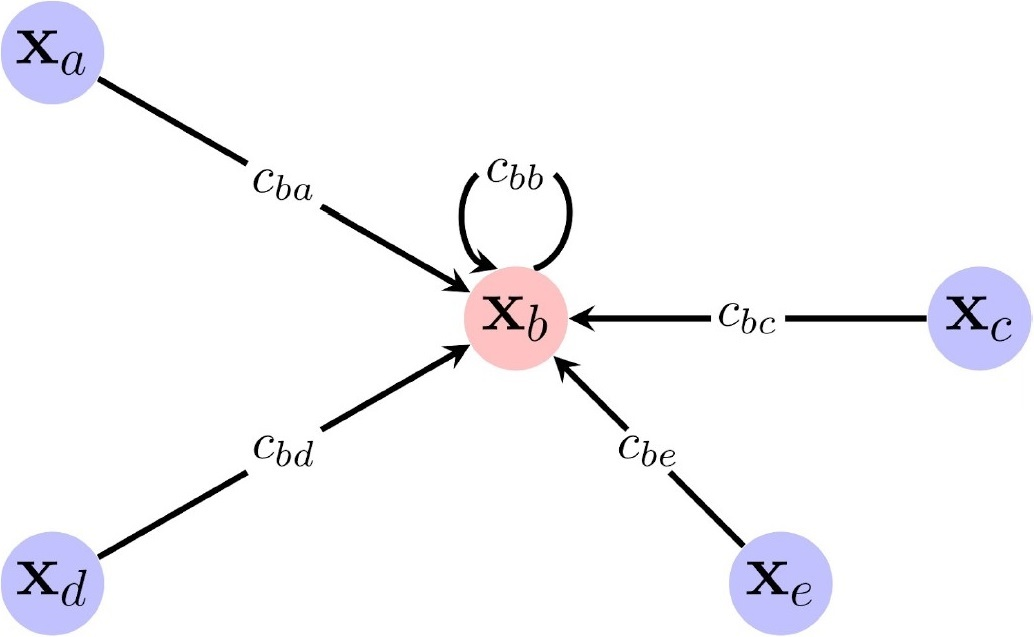
\includegraphics[width=\textwidth]{figs/convolutional-gnn}
			\caption{Convolutional}
			\label{fig:convolutional-gnn}
		\end{subfigure}
		\begin{subfigure}[b]{0.3\textwidth}
			\centering
			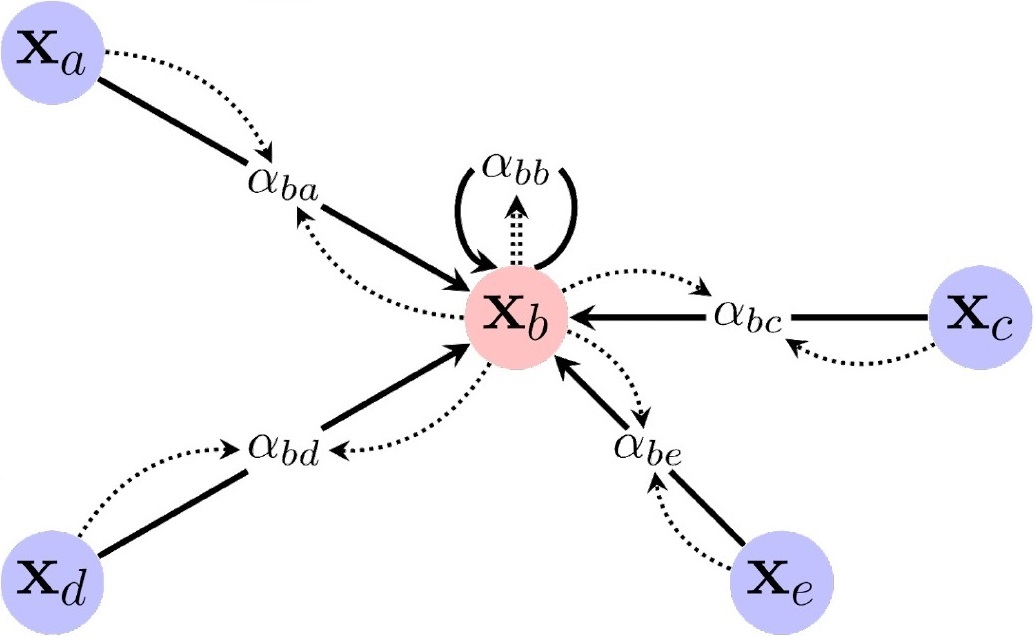
\includegraphics[width=\textwidth]{figs/attentional-gnn}
			\caption{Attentional}
			\label{fig:attentional-gnn}
		\end{subfigure}
		\begin{subfigure}[b]{0.3\textwidth}
			\centering
			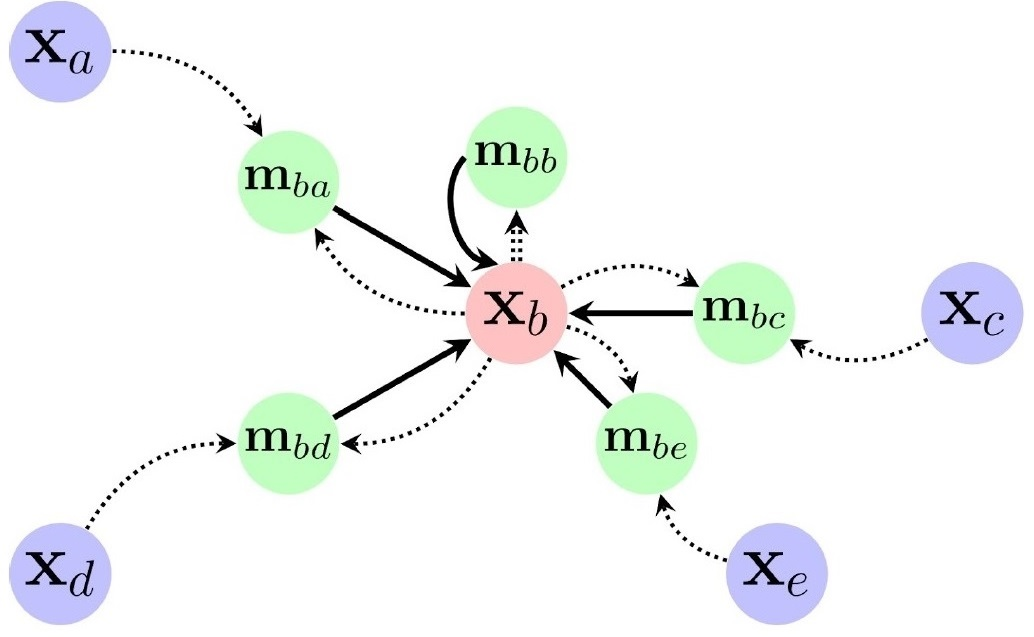
\includegraphics[width=\textwidth]{figs/message-passing-gnn}
			\caption{Message-passing}
			\label{fig:message-passing-gnn}
		\end{subfigure}
	\end{figure}
	\vspace*{-1.5\baselineskip}
	$$\begin{array}{ccc}
		\hspace*{-3em}\mathbf{h}_i=\phi\left(\mathbf{x}_i,\displaystyle\bigoplus_{j\in\mathcal{N}_i}c_{ij}\psi(\mathbf{x}_j)\right) & 
		\mathbf{h}_i=\phi\left(\mathbf{x}_i,\displaystyle\bigoplus_{j\in\mathcal{N}_i}a(\mathbf{x}_i,\mathbf{x}_j)\psi(\mathbf{x}_j)\right) &
		\mathbf{h}_i=\phi\left(\mathbf{x}_i,\displaystyle\bigoplus_{j\in\mathcal{N}_i}\psi(\mathbf{x}_i,\mathbf{x}_j)\right)
	\end{array}$$
	
	\item Convolutional GNNs:
	\begin{itemize}[topsep=0pt]
		\item Graph Convolutional Network (GCN; \href{https://openreview.net/pdf?id=SJU4ayYgl}{Kipf \& Welling, ICLR 2017}):
		$$\mathbf{H}=\sigma\left(\tilde{\mathbf{D}}^{-\frac{1}{2}}\tilde{\mathbf{A}}\tilde{\mathbf{D}}^{-\frac{1}{2}}\mathbf{X}\mathbf{W}\right)$$
		where $\tilde{\mathbf{A}}=\mathbf{A}+\mathbf{I}$, and $\tilde{\mathbf{D}}$ is the corresponding degree matrix of $\tilde{\mathbf{A}}$
		\item Simplified Graph Convolution (SGC; \href{http://proceedings.mlr.press/v97/wu19e/wu19e.pdf}{Wu \textit{et al.}, ICML 2019}):
		$$\mathbf{H}=\text{Softmax}\left(\left(\tilde{\mathbf{D}}^{-\frac{1}{2}}\tilde{\mathbf{A}}\tilde{\mathbf{D}}^{-\frac{1}{2}}\right)^K\mathbf{X}\mathbf{W}\right)$$
		Near state-of-the-art on many tasks of interest, and very efficient to train
		\item Chebyshev Networks (ChebyNet; \href{https://papers.nips.cc/paper/2016/file/04df4d434d481c5bb723be1b6df1ee65-Paper.pdf}{Defferrard \textit{et al.}, NIPS 2016}):
		$$\mathbf{H}=\sigma\left(\sum_{k=0}^K\alpha_k\left(\frac{2}{\lambda_\text{max}}\mathbf{L}_\text{sym}-\mathbf{I}\right)^k\mathbf{X}\mathbf{W}_k\right)$$
		where 
		\begin{itemize}[topsep=0pt]
			\item $\lambda_\text{max}$ is the largest eigenvalue of $\mathbf{L}_\text{sym}$ 
			\item $\alpha_k$ is the order-$k$ coefficient of its Chebyshev polynomial
		\end{itemize}
		GCN can be interpreted as a ChebyNet with $K=1$ and $\lambda_\text{max}\approx2$
	\end{itemize}
	
\end{enumerate}

\newpage

\subsection*{Appendix: Mathematical Notations}

\renewcommand\arraystretch{1.5}
\begin{tabular}{p{2cm}p{12cm}}
	$\displaystyle a$ & A scalar (integer or real) \\
	$\displaystyle \mathbf{a}$ & A vector \\
	$\displaystyle \mathbf{A}$ & A matrix \\
	$\displaystyle \mathcal{A}\text{ or }\{\cdot\}$ & A set \\
	$\displaystyle \{\!\{\cdot\}\!\}$ & A multiset \\
	$\displaystyle |\mathcal{A}|$ & Cardinality of set $\mathcal{A}$ \\
	$\displaystyle \mathbb{R}$ & The set of real numbers \\
	$\displaystyle a_i$ & Element $i$ of vector $\mathbf{a}$, with indexing starting at 1 \\
	$\displaystyle A_{ij}$ & Element $i$, $j$ of matrix $\mathbf{A}$, with indexing starting at 1 \\
	$\displaystyle f$ & A function \\
	$\displaystyle \bm{F}$ & A matrix-valued function \\
	$\displaystyle \pi$ & A permutation \\
	$\displaystyle \phi, \psi, \rho, \cdots$ & Learnable functions (e.g., MLPs) \\
	$\displaystyle \sigma$ & A non-linear activation function (e.g., sigmoid, ReLU) \\
	$\displaystyle \oplus$ & A permutation-invariant operator (e.g., sum, mean, min, max)
\end{tabular}

\end{document}
